\documentclass[a4paper,12pt]{article}
\usepackage{graphicx}
\usepackage{float}
\usepackage{hyperref}
\usepackage{geometry}
\usepackage{titlesec}
\usepackage{tikz}
\usepackage{pgfplots}
\usepackage{pgf-pie}
\pgfplotsset{compat=1.17}
\geometry{margin=1in}

\titleformat{\section}{\large\bfseries}{\thesection}{1em}{}

\title{OEE Report \\ \large Tulip Application Development Virtual Internship \\ Final Report}
\author{Pranav Verma}
\date{\today}

\begin{document}

\maketitle
\tableofcontents
\newpage

\section{Executive Summary}

This report presents the finalized version of a customized OEE (Overall Equipment Effectiveness) report developed using Tulip's low-code platform. The primary objective was to design, build, and refine a real-time production monitoring dashboard that accurately tracks machine availability, performance, and quality. Through iterative development, real production data integration, testing, and feedback-based refinements, the resulting report provides actionable insights to support production teams in enhancing operational efficiency.

\vspace{0.5cm}
\noindent\textbf{Key Features:}

The report features real-time data integration from machine logs and production sensors, providing up-to-the-minute information. It includes clear visualizations in the form of graphs, tables, and charts that enable effective data interpretation. The dashboard focuses on three critical metrics: Availability, Performance, and Quality. Additionally, the design is user-friendly and has been optimized based on comprehensive usability testing and valuable mentor feedback.

\section{Introduction and Objective}

The purpose of the OEE report is to monitor and analyze production efficiency, ensuring that manufacturing processes are optimized for maximum output and minimal downtime. The objective is to develop a customized, functional OEE report using Tulip's low-code platform that integrates live production data and presents it in a user-centric, actionable format.

\section{Report Structure and Key Features}

\subsection{Layout Overview}

The report layout is divided into three primary sections. The Summary Dashboard displays the overall OEE score and breakdowns, providing a high-level view of production efficiency. The Detailed Metrics section delves deeper into Availability, Performance, and Quality, offering trend analysis for each component. Finally, the Historical Data section presents graphs showing daily, weekly, and monthly performance trends, enabling long-term performance tracking and pattern recognition.

\subsection{Integrated Real-Time Data}

The report is connected to machine sensors and production databases via Tulip connectors, ensuring live updates for key metrics.

\subsection{Key Performance Metrics}

The report tracks three essential OEE components. Availability measures machine uptime versus planned production time, highlighting periods of unexpected downtime or maintenance issues. Performance compares actual production speed to ideal production speed, identifying slowdowns and inefficiencies in the manufacturing process. Quality assesses the ratio of good units produced versus total units, tracking defect rates and production accuracy.

% Structure Diagram via TikZ
\begin{figure}[H]
    \centering
    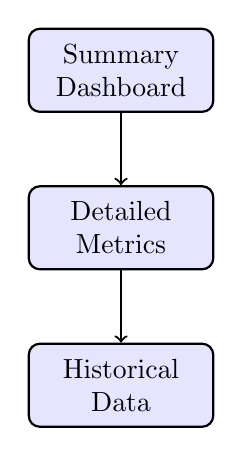
\begin{tikzpicture}[node distance=2cm, auto, thick]
        \tikzstyle{block} = [rectangle, draw, fill=blue!10, text width=6em, text centered, rounded corners, minimum height=3em]
        \node[block] (summary) {Summary Dashboard};
        \node[block, below of=summary] (detailed) {Detailed Metrics};
        \node[block, below of=detailed] (historical) {Historical Data};
        \draw[->] (summary) -- (detailed);
        \draw[->] (detailed) -- (historical);
    \end{tikzpicture}
    \caption{Customized OEE Report Structure}
\end{figure}

\section{Data Sources and Visualizations}

\subsection{Data Sources}

The OEE report draws from multiple data streams to ensure comprehensive monitoring. Machine logs capture detailed information about machine start and stop times, providing critical data for availability calculations. Sensor data enables real-time cycle time and downtime monitoring, ensuring accurate performance metrics. The production database records the number of good and defective units produced, which is essential for quality assessment and overall OEE calculation.

\subsection{Visualizations}

The report incorporates several types of visualizations to present data effectively. Line charts display OEE trends over time, making it easy to identify patterns and changes in overall efficiency. Bar charts compare Availability, Performance, and Quality metrics across different shifts, facilitating cross-shift analysis and identification of best practices. Pie charts break down downtime causes, helping teams quickly identify the most significant factors affecting machine availability and prioritize improvement efforts.

% OEE Trend Line Chart via PGFPlots
\begin{figure}[H]
    \centering
    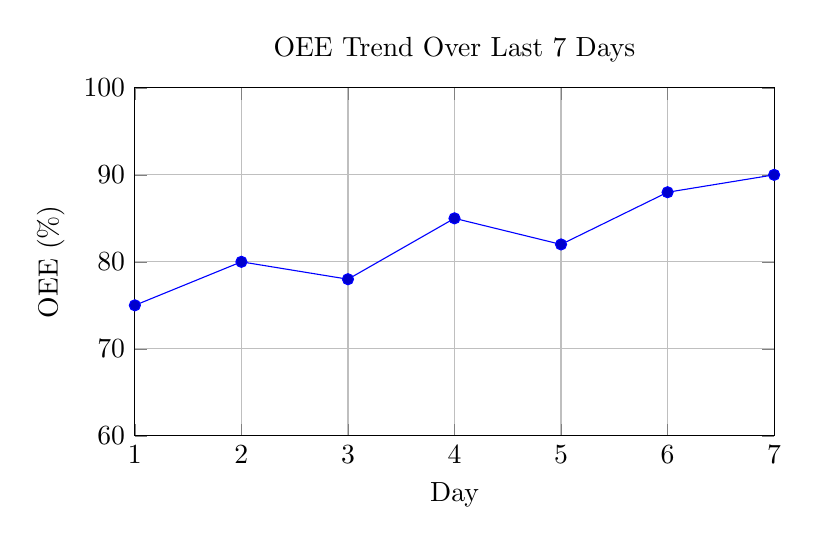
\begin{tikzpicture}
    \begin{axis}[width=0.8\textwidth, height=6cm,
        title={OEE Trend Over Last 7 Days},
        xlabel={Day}, ylabel={OEE (\%)},
        xmin=1, xmax=7, ymin=60, ymax=100,
        xtick={1,2,3,4,5,6,7},
        ytick={60,70,80,90,100},
        grid=major]
    \addplot coordinates {(1,75) (2,80) (3,78) (4,85) (5,82) (6,88) (7,90)};
    \end{axis}
    \end{tikzpicture}
    \caption{Sample OEE Visualization: OEE Trend Over Time}
\end{figure}

% Pie Chart via pgf-pie
\begin{figure}[H]
    \centering
    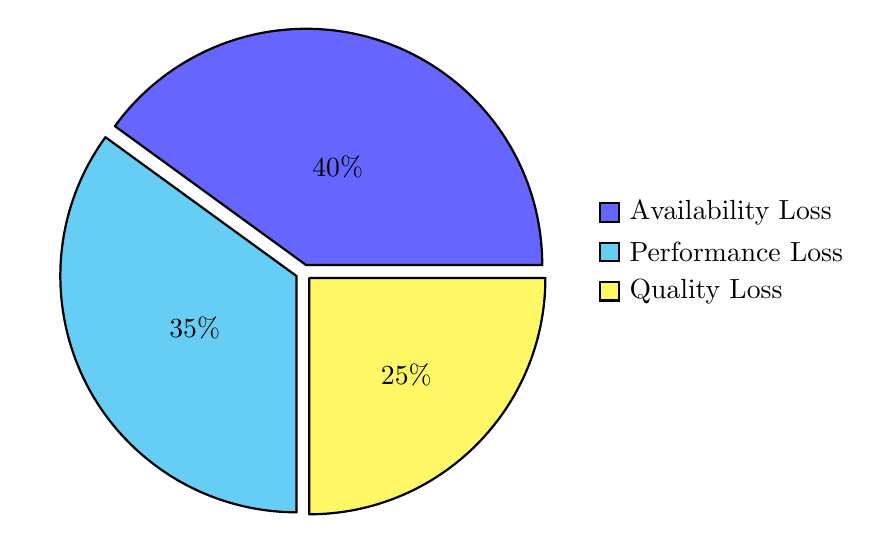
\begin{tikzpicture}
    \pie[text=legend, explode=0.1]{40/Availability Loss, 35/Performance Loss, 25/Quality Loss}
    \end{tikzpicture}
    \caption{Downtime Cause Breakdown}
\end{figure}

\section{Testing and Accuracy Checks}

\subsection{Testing Process}

A rigorous testing approach was implemented to ensure report reliability. Data from the report was cross-verified with manual production records to confirm accuracy and consistency. End-to-end workflow testing was conducted using test production runs to validate data flow and calculation integrity. Additionally, users from production teams were actively engaged to interact with the report, providing practical feedback on usability and functionality from those who would rely on it daily.

\subsection{Accuracy and Usability Assurance}

To ensure report reliability, accuracy checks identified and corrected mismatches between sensor data and report output, guaranteeing that the displayed metrics accurately reflect actual production conditions. From a usability perspective, navigation was simplified, labeling was improved, and mobile responsiveness was ensured, making the report accessible and functional across different devices and user scenarios.

\section{Feedback and Improvements}

\subsection{Feedback Summary}

Feedback was collected through multiple channels to gain comprehensive insights. Usability sessions allowed direct observation of how users interacted with the interface. Direct interviews provided in-depth feedback about specific features and pain points. Walkthrough demonstrations helped identify areas where the report's flow could be improved or where additional information was needed.

\subsection{Key Improvements Implemented}

Several key improvements were implemented based on collected feedback. Visualization enhancement added color-coding for quick interpretation, making it easier to identify issues at a glance. Data granularity was improved by introducing hourly views alongside daily summaries, providing more detailed insights for troubleshooting. Error handling was strengthened with notifications for missing or delayed sensor data, ensuring users are aware of any potential data integrity issues. Navigation was improved through hyperlinked sections for faster access within the dashboard, allowing users to quickly move between related data points.

\section{Implementation Plan and Next Steps}

\subsection{Usage by Production Teams}

The OEE report is designed to support production teams through multiple use cases. It enables daily monitoring during production shifts, allowing real-time response to efficiency issues. The report facilitates weekly and monthly OEE reporting for management review, supporting strategic decision-making and resource allocation. Additionally, it provides data for root cause analysis of downtime, allowing teams to identify and address recurring issues based on captured data trends.

\subsection{Future Improvements}

Several enhancements are planned for future iterations of the OEE report. Integration of predictive analytics will enable forecasting of potential downtimes, allowing preventive action before issues occur. Machine learning modules will be added for anomaly detection, automatically flagging unusual patterns that may indicate developing problems. The dashboard scope will be expanded to cover multiple production lines simultaneously, providing a comprehensive view of facility-wide efficiency.

\section{Final Version of Customized OEE Report}

% Dashboard Overview via TikZ and PGFPlots
\begin{figure}[H]
    \centering
    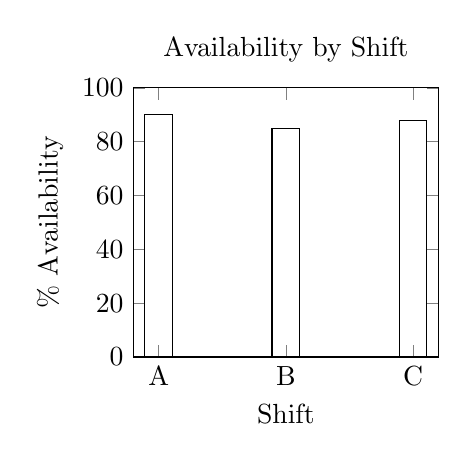
\begin{tikzpicture}
    \begin{axis}[width=0.45\textwidth, height=5cm, title={Availability by Shift},
        xlabel={Shift}, ylabel={\% Availability},
        symbolic x coords={A, B, C}, xtick=data, ymin=0, ymax=100]
      \addplot[ybar] coordinates {(A,90) (B,85) (C,88)};
    \end{axis}
    \end{tikzpicture}
    \quad
    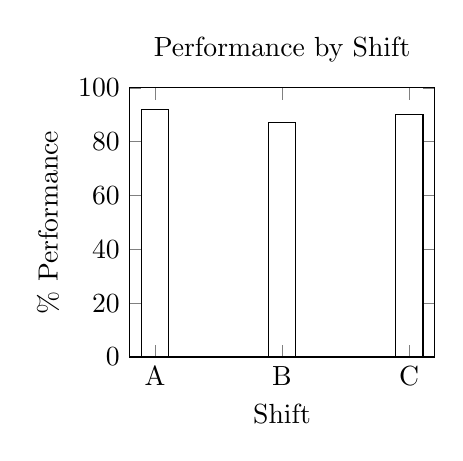
\begin{tikzpicture}
    \begin{axis}[width=0.45\textwidth, height=5cm, title={Performance by Shift},
        xlabel={Shift}, ylabel={\% Performance},
        symbolic x coords={A, B, C}, xtick=data, ymin=0, ymax=100]
      \addplot[ybar] coordinates {(A,92) (B,87) (C,90)};
    \end{axis}
    \end{tikzpicture}
    \caption{Availability and Performance by Shift}
\end{figure}

\begin{figure}[H]
    \centering
    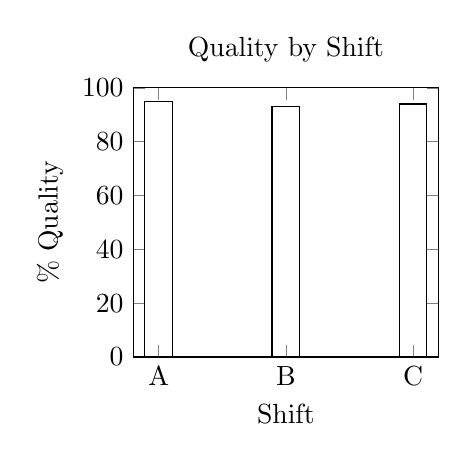
\begin{tikzpicture}
    \begin{axis}[width=0.45\textwidth, height=5cm, title={Quality by Shift},
        xlabel={Shift}, ylabel={\% Quality},
        symbolic x coords={A, B, C}, xtick=data, ymin=0, ymax=100]
      \addplot[ybar] coordinates {(A,95) (B,93) (C,94)};
    \end{axis}
    \end{tikzpicture}
    \quad
    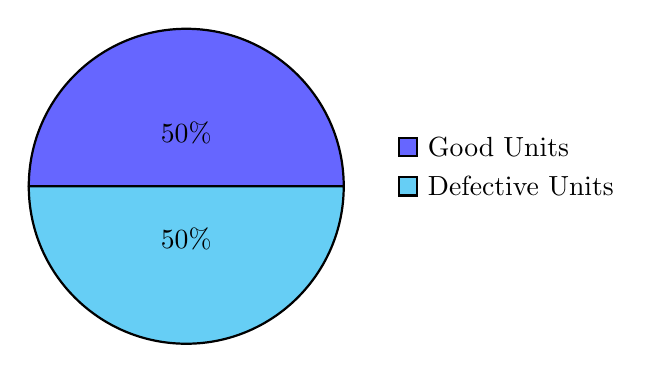
\begin{tikzpicture}
    \pie[text=legend, radius=2]{50/Good Units, 50/Defective Units}
    \end{tikzpicture}
    \caption{Quality by Shift and Units Production Breakdown}
\end{figure}

\section*{Conclusion}

The development of the Customized OEE Report involved building, testing, and refining a robust production monitoring tool. By leveraging Tulip's low-code capabilities and real-time data integration, the resulting report not only meets production monitoring needs but also empowers teams to drive continuous improvements based on clear, actionable insights.

\vspace{0.5cm}
\noindent\textbf{Submitted By:} \\
Pranav Verma \\
Tulip Application Development Virtual Internship - Week 5

\end{document}
